\chapter{Processamento de Formulários}
\epigraph{``\textit{O modo como você reúne, administra e usa a informação determina se vencerá ou perderá.}''.}{Bill Gates}

\lettrine[lines=4, lhang=0.1, lraise=0, loversize=0.2, findent=0.1em]{\textcolor{corAzulTema}{N}}{ESTE} Capítulo teremos como objetivos entender o funcionamento de formulários HTML e conseguirmos diferenciar os métodos do protocolo HTTP e como tratá-los.


\section{Introdução}

Neste Capítulo vamos começar a aprender a criar algo útil! No Capítulo anterior, aprendemos as bases do desenvolvimento Web em Java, criamos alguns programas de brinquedo\footnote{Programa de brinquedo é todo programa criado para apresentar algum conceito e que, normalmente, não tem uma utilidade prática além da pedagógica.} para aplicar as técnicas que aprendemos e agora vamos aprender mais alguns detalhes, mas dessa vez nossos programas serão mais elaborados. Vamos começar?


\section{Formulários}

A forma tradicional de se desenvolver aplicações para Web que interajam com o servidor é utilizando os chamados formulários. Um formulário é composto normalmente por um conjunto de componentes que permitem que o usuário forneça dados para serem submetidos ao servidor. Quando esses dados são recebidos pelo servidor, algum componente da aplicação vai tratá-los, sendo que no nosso caso, esse componente vai ser implementado na forma de um Servlet.
Atualmente existem diversas técnicas para a criação de aplicações Web, sendo que, dependendo da técnica/tecnologia, a forma de submeter dados ao servidor é diferente. Uma dessas técnicas é o chamado Asynchronous JavaScript and XML (AJAX) que hoje em dia é implementado de inúmeras formas. Neste livro não iremos aprender a usar AJAX, porque infelizmente não teremos tempo, mas garanto que se você se empenhar no decorrer do nosso curso, ao final, você estará apto a aprender a trabalhar com AJAX.

Abra o NetBeans e crie um novo projeto Java Web. Dê o nome de ``PrimeiroFormulario'' (sem as aspas). Sempre que for criar um novo projeto, siga os passos descritos na Subseção \label{subsec:primeiroProjeto} do Capítulo 1. Com o projeto criado, vamos editar o \texttt{index.html}. Nele vamos alterar o título da página e criar nosso primeiro formulário, que será usado para preenchermos dados pessoais de um cliente. Veja na Listagem~\thechapter.\ref{listagem:projetos/capitulo02/PrimeiroFormulario/web/index.html} como ficou o código. Não se esqueça de copiá-lo no seu \texttt{index.html}.

\htmlCode{Protótipo do formulário de dados do cliente (\texttt{index.html})}{projetos/capitulo02/PrimeiroFormulario/web/index.html}

Copiou? Salve o arquivo e execute a aplicação. Você vai ter algo como o mostrado na Figura~\ref{fig:cap02PrimeiroFormulario}.

\FloatBarrier
\begin{figure}[!htbp]
    \centering
    \caption{Visualização do protótipo do formulário de dados do cliente}
    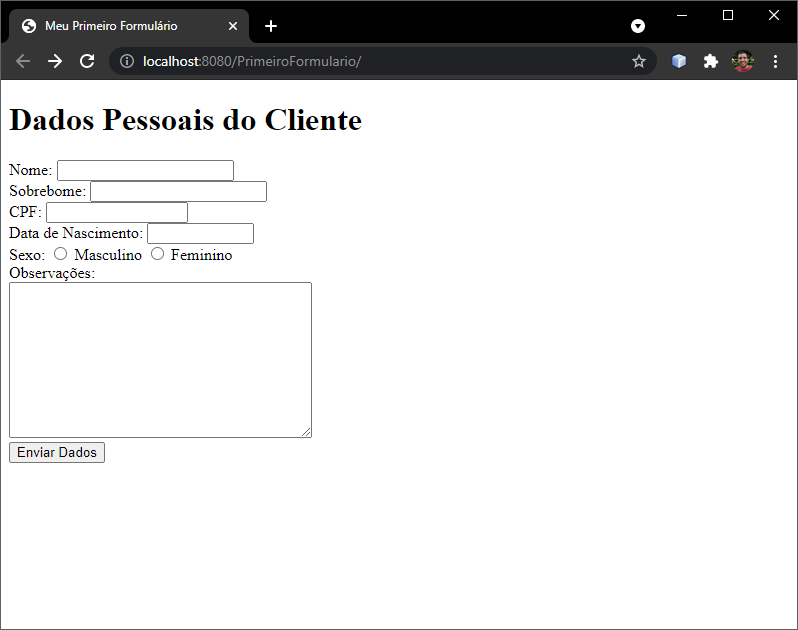
\includegraphics[scale=0.7]{imagens/cap02PrimeiroFormulario}
    \\\textbf{Fonte:} Elaborada pelo autor
    \label{fig:cap02PrimeiroFormulario}
\end{figure}
\FloatBarrier

Quanta coisa! O formulário não ficou uma obra prima, mas esse não é nosso objetivo agora. Precisamos entender o que cada \textit{tag} faz. Vamos agora analisar o código da Listagem~\thechapter.\ref{listagem:projetos/capitulo02/PrimeiroFormulario/web/index.html} e entender o protótipo que fizemos. Irei detalhar apenas as \textit{tags} \texttt{<form>} e seus componentes, pois acredito que você já conheça as outras que foram utilizadas. Vamos lá então:

\begin{itemize}
    \item \textbf{Linha 13:} Nesta linha abrimos a \textit{tag} \texttt{<form>} que delimita um formulário HTML. Note que fechamos a \textit{tag} form na linha 43. Todas as \textit{tags} que forem inseridas entre \texttt{<form>} e \texttt{</form>} farão parte do formulário;
    
    \item \textbf{Linha 15:} Criamos um \textit{label} (tag <label>) com o conteúdo ``Nome: ''. A \textit{tag} \texttt{<label>} é usada para criar um rótulo. Ao invés de usar a \textit{tag} \texttt{<label>}, poderíamos simplesmente ter inserido o texto que queremos mostrar no formulário, mas como o texto que estamos utilizando tem o propósito de ser um rótulo para um campo do formulário, iremos utilizar essa tag para deixar nosso código mais organizado e inserir uma certa carga semântica no nosso código;
    
    \item \textbf{Linha 16:} Criamos um \textit{input} (campo de entrada) do tipo \textit{text} (texto) com tamanho de 20 colunas e com o nome de ``nome''. Dentre as \textit{tags} que representam componentes nos formulários, a \texttt{<input>} é uma delas. Existem vários tipos de \textit{inputs}, diferenciados pela propriedade \texttt{type}, e que vamos aprender aos poucos. A propriedade \texttt{size}, como você deve ter percebido, é utilizada para configurar a largura do campo de texto. A propriedade \texttt{name} é utilizada pelo navegador para identificar os dados do componente em questão no momento de enviar os dados para o servidor. Não entendeu a utilidade da propriedade \texttt{name}? Não se preocupe, logo vai fazer sentido;
    
    \item \textbf{Linha 17:} Usamos a \textit{tag} \texttt{<br/>} para pular uma linha;
    
    \item \textbf{Linhas 19 a 29:} Os próximos três campos (sobrenome, CPF e data de nascimento) são bem parecidos com o primeiro;
    
    \item \textbf{Linha 32:} Criamos um input do tipo \textit{radio} (botão de rádio), com nome configurado como ``sexo'' e com o valor (\texttt{value}) configurado com ``M'';
    
    \item \textbf{Linha 33:} Idem à linha anterior, com a diferença que o valor é ``F''. Note que a propriedade name de ambos os radios é a mesma, pois eles representam o mesmo campo (sexo). Perceba que no navegador, se você selecionar um deles e depois clicar no outro, o que estava selecionado previamente deixa de ser selecionado. Se a propriedade \texttt{name} for diferente, eles serão considerados campos diferentes e então esse comportamento da seleção não existirá. Note ainda que você pode ``amarrar'' quantos radios você precisar;
    
    \item \textbf{Linha 38:} Nessa linha definimos uma área de texto. Esse componente, representado pela \textit{tag} textarea é utilizado, como o próprio nome já diz, para criar uma área de texto livre, onde o usuário poderá digitar uma quantidade arbitrária de texto. Note que para utilizar um textarea nós precisamos usar a \textit{tag} de fechamento (<textarea>), ao invés de fazer da forma que estamos fazendo com os inputs. A novidade nesse componente são as propriedades cols e rows, que são usadas respectivamente para definir a quantidade de colunas e de linhas do componente;
    
    \item \textbf{Linha 41:} Por fim, nessa linha definimos um input do tipo submit, que é um botão que tem o comportamento padrão de, ao ser clicado, submeter (enviar) os dados do formulário para o servidor. Note que usamos a propriedade value para definir o texto do botão.
\end{itemize}

Agora que já conhecemos alguns dos componentes que podemos utilizar nos nossos formulários, mas você deve estar se perguntando: ``Tudo bem, o input do tipo submit é usado para enviar os dados do formulário para o servidor, mas onde eu digo ao submit para onde os dados do formulário devem ser enviados?''. Vamos à resposta!
Eu tenho dito várias vezes que o componente que vai tratar os dados de um formulário na nossa aplicação é o Servlet não é mesmo? Então precisamos criar um Servlet que vai receber esses dados e então configurar o formulário para direcionar os dados inseridos nele para o Servlet apropriado.
Vamos criar o Servlet? Mas agora iremos fazer de uma forma mais automática do que a que estamos fazendo desde que aprendemos a trabalhar com os Servlets. Na pasta de pacotes de código-fonte do projeto, crie um pacote chamado ``primeiroformulario.servlets'' (sem as aspas). Clique com o botão direito no pacote criado, escolha ``Novo'' e procure pela opção ``Servlet...''. Se não encontrou, escolha a propriedade ``Outro...'', selecione ``Web'' na categoria, ``Servlet'' no tipo de arquivo e clique em ``Próximo''. 
Preencha o campo ``Nome da classe'' com ``ProcessaDadosClienteServlet'' (sem as aspas) e clique em ``Próximo''. Nesse passo, note que o assistente nos pede o nome do Servlet e o padrão de URL. Lembra que criávamos nossa classe do Servlet e implementávamos seu esqueleto, além de fazer seu mapeamento no DI, manualmente? Agora o NetBeans vai fazer tudo isso para nós automaticamente! Deixe o campo ``Nome do Servlet'' com o valor padrão (que é o nome da classe) e preencha o campo ``Padrão(ões) de URL'' com ``/processaDadosCliente'' (sem as aspas). Não iremos aprender sobre os padrões de inicialização na nossa disciplina, mas nada impede que você aprenda para que eles servem, basta consultar a bibliografia recomendada nas referências bibliográficas da apostila tudo bem? Tudo feito? Clique em ``Finalizar''.
Ao fazer isso, o nosso Servlet será criado e aberto no editor. Como eu sei que você é uma pessoa super curiosa, dê uma olhada no web.xml para ver que o Servlet que foi criado já foi mapeado lá! Legal hein?
Note que o NetBeans já implementou o esqueleto do Servlet para nós. O primeiro método implementado é o processRequest. Lembra-se dele? É nele que vamos inserir o código que queremos que o Servlet execute. Após o fechamento do bloco deste método, note que existe uma linha onde está escrito ``HttpServlet methods. Click on the + sign on the left to Edit the code.''. Siga a sugestão da frase e clique no ``+''. O que apareceu? A implementação dos métodos GET e POST, sendo que dentro delas é chamado o processRequest! Viu só? Da mesma forma que fazíamos manualmente! Não iremos mexer ali, então você pode contrair novamente esta seção do código clicando no sinal de ``–''.
Note que além de implementar o esqueleto do nosso Servlet, o NetBeans também inseriu um trecho de código dentro do processRequest. O código que está inserido configura o tipo de retorno do Servlet (response.setContentType(...)), obtém o canal de escrita do Servlet, escreve uma série de Strings que representam uma página HTML nesse canal e o fecha. Você se lembra que já falei algumas vezes que não iremos implementar Servlets que geram código HTML? Então, vamos limpar esse método, tirando todo o código que foi inserido dentro dele. Vá no editor e apague o conteúdo entre as linhas 30 (response.setContentType(...)) e 45 (``\}''), incluindo elas. Seu processRequest deve estar vazio agora.
Antes de codificarmos, vamos a mais um pouquinho de teoria. Você se lembra, lá no comecinho da primeira aula, que eu falei que o cliente manda uma requisição para o servidor e ele manda uma resposta? Nos Servlets, essa requisição e essa resposta são representadas respectivamente por objetos do tipo HttpServletRequest e HttpServletResponse. Note que os três métodos implementados nos nossos Servlets (processRequest, doGet e doPost) recebem dois parâmetros, sendo eles dos tipos que mencionei. Qual a conclusão que você chega então? Os dados enviados pelo cliente ao servidor estão dentro do objeto do tipo HttpServletRequest, que chamamos de request no nosso código e os dados que enviamos de volta ao cliente devem ser inseridos no objeto do tipo HttpServletResponse, que demos o nome de response.
Sabendo disso, agora ficou fácil! Os dados do formulário de clientes que estamos construindo serão recebidos pelo nosso Servlet através do objeto apontado por request! Legal não é? Mas ainda falta um detalhe... Não informamos ao formulário para quem ele deve enviar os dados! Vamos fazer isso agora. Volte no index.jsp e procure pela \textit{tag} form (a mesma que está na linha 15 da Listagem 2.1). Para informarmos à \textit{tag} form qual é o destino dos seus dados, utilizamos a propriedade action, sendo que nesta propriedade, colocamos a URL do componente que deve tratar os dados do formulário. Mapeamos nosso Servlet usando o padrão ``/processaDadosCliente'' não foi? Então, qual será a URL do nosso Servlet? Resposta: ``http://localhost:8084/PrimeiroFormulario/processaDadosCliente''. Vamos editar nossa \textit{tag} form então, configurando a propriedade action para a URL citada. Na Listagem 2.2 você pode ver como ficou o código da \textit{tag} form. Note que não estou listando todo o arquivo.

Listagem 2.2: Configurando a propriedade action da \textit{tag} form
 
Fonte: do autor
Isso que dizer que, quando clicarmos no botão ``Enviar Dados'' (que é um input do tipo submit), os dados que estiverem preenchidos nos componentes que estão dentro deste formulário, serão enviados para http://localhost:8084/PrimeiroFormulario/processaDadosCliente, que é o endereço do nosso Servlet! Já alterou o arquivo? Salvou? Legal! Atualize a página, preencha os campos e clique no botão ``Enviar Dados''. O que aconteceu? Uma página em branco foi exibida não é? E na barra de endereços, o que apareceu? O endereço do Servlet mais um monte de ``coisas''! Os detalhes sobre isso nós iremos aprender na próxima seção, então não se preocupe por enquanto.
Você se lembra dos nossos primeiros exemplos? Acessávamos o endereço do Servlet, uma página em branco era exibida e duas Strings eram direcionadas para a saída do Tomcat, lembra? Quem fazia esse direcionamento era o Servlet não era? Vamos fazer a mesma coisa com o nosso Servlet de dados dos clientes, mas mostraremos os dados que foram preenchidos nos formulários. Vamos lá então?
Volte ao Servlet, vamos implementar o método processRequest. Qual é mesmo o nome do parâmetro do método processRequest que armazena os dados enviados pelo cliente? É o request certo? Veja o código da Listagem 2.3. Leia o comentário que fiz.













Listagem 2.3: Implementação do método processRequest
 
Fonte: do autor
Copiou o código? Legal. Vamos entender o que está acontecendo. Na linha 14 é declarada uma variável do tipo String com o nome de ``nome''. Essa variável é inicializada com o valor obtido ao se chamar o método getParameter( String param ) de request. O parâmetro passado ao método getParameter, que é uma String, é o nome que foi dado ao componente do formulário, que no caso foi ``nome''. Estude as linhas 15, 16, 17, 18 e 19 e tente fazer um paralelo com o formulário contido no index.jsp. Note que a String que é passada como parâmetro no método getParameter(...) sempre reflete o nome dado ao componente do formulário através da propriedade name. Veja a linha 17. Declaramos uma variável chamada dataNascimento que é inicializada com o valor do parâmetro ``dataNasc'' (configurado no formulário).
O que fizemos até a linha 19 foi criar uma variável que vai receber o valor de cada componente do formulário. A partir da linha 21, até o final do método, direcionamos para a saída os dados que foram obtidos. Vamos testar? Salve o Servlet e execute o projeto (botão de ``play'', lembra?). Na página, preencha o formulário, clique em ``Enviar Dados'' e volte no NetBeans para ver o que aconteceu. Olhe na janela de saída! Lá estão os dados que você preencheu no formulário! Muito bem! Imagine agora se esse fosse um sistema real. Esses dados recebidos dentro do Servlet poderiam alimentar uma query SQL para inserir esse cliente em um banco de dados! Legal não é?! A partir desse ponto, você já deve estar entendendo melhor o que está acontecendo não é mesmo? Mas e aquele monte de coisas escritas no endereço do navegador depois de clicar em Enviar Dados? Esse comportamento está intrinsecamente ligado ao tipo de método HTTP que estamos usando. Vamos para a próxima seção, vou explicar isso lá.


\section{Métodos HTTP}

O protocolo HTTP 1.1, que usamos em nossas aplicações Web, define uma série de métodos que podem ser usados para tratar diversos tipos de requisições. Na nossa vida, como desenvolvedores Web, iremos nos importar somente com os métodos GET e POST. Sendo assim vamos detalhá-los.
<Saiba mais:
Quer conhecer os outros métodos HTTP (HEAD, TRACE, etc.)? Acesse este link: http://www.w3.org/Protocols/rfc2616/rfc2616-sec9.html (em inglês)
>


\subsection{Método GET}

O método GET (to get = obter) é usado principalmente para pedir ao servidor algum recurso. Quando nós fazemos uma pesquisa no Google, por exemplo, estamos usando o método GET. Qualquer URL que colocamos na barra de endereço do nosso navegador é enviada ao servidor usando o método GET. Vamos fazer um teste. Entre na página do Google (www.google.com.br) e pesquise por ``métodos http'' (sem as aspas). Ao clicar em pesquisar, o resultado será mostrado no navegador. Veja a barra de endereços. Haverá algo assim:
%\url{http://www.google.com.br/#hl=pt-BR\&biw=1440\&bih=713\&q=métodos+http\&aq=f\&
%aqi=g10\&aql=\&oq=\&gs_rfai=\&fp=90f65ad7da748e6d}
Parece grego, mas não é! Vamos entender a URL. Estamos usando o protocolo HTTP, para acessar a máquina www.google.com.br. O recurso é representado pelo restante da URL:
%hl=pt-BR\&biw=1440\&bih=713\&q=métodos+http\&aq=f\&aqi=g10\&aql=\&oq=\&gs_rfai=\&
fp=90f65ad7da748e6d
Vamos dividir esse resto da URL nos símbolos ``\&''. Vamos obter isso aqui:
hl=pt-BR
biw=1440
bih=713
q=métodos+http
aq=f
aqi=g10
...
Note que a forma de cada pedaço da parte correspondente ao recurso é x=y, onde ``x'' é o nome de uma variável e ``y'' é o valor. No nosso exemplo, a variável ``q'' tem o valor ``métodos+http'' que no caso é a nossa consulta! Ou seja, o componente que trata as pesquisas do Google, entende que a variável ``q'' vai conter o valor da pesquisa que estamos fazendo!
Execute novamente o nosso projeto, limpe todos os campos e preencha o campo ``Nome'' com ``Juca'' (sem as aspas) e o campo ``Sexo'' com Masculino e clique em ``Enviar Dados''. Veja a URL que foi obtida na barra de endereços:
%T\url{http://localhost:8084/PrimeiroFormulario/processaDadosCliente?nome=Juca&
%sobrenome=&cpf=&dataNasc=&sexo=M&observacoes=}
Veja o caminho do recurso!
%processaDadosCliente?nome=Juca\&sobrenome=\&cpf=\&dataNasc=\&sexo=M\&observacoes=
O que isso quer dizer:
Senhor ``processaDadosCliente'', por favor, receba as variáveis nome, sobrenome, cpf, dataNasc, sexo e observacoes, utilize seus valores e me devolva o recurso associado a eles. O ponto de interrogação após o mapeamento do Servlet (/processaDadosCliente) indica que o que vem depois dele (do ponto de interrogação) são variáveis HTTP. Cada variável, como já vimos, está na forma x=y, onde ``x'' é a variável e ``y'' é o valor, sendo que elas são separadas por ``\&''. Então temos: ``nome'' igual a ``Juca'', ``sobrenome'' igual a vazio, ``cpf'' igual a vazio, ``dataNasc'' igual a vazio, ``sexo'' igual a ``M'' e ``observacoes'' igual a vazio. A saída no NetBeans deve ter ficado assim:
Dados do Cliente:
Nome: Juca
Sobrenome: 
CPF: 
Data de Nascimento: 
Sexo: Masculino
Observações:
Vamos mandar a requisição novamente para o NetBeans, só que agora modificando a URL ao invés de usar o formulário. Dê o sobrenome de ``Santos'' ao Juca e defina o CPF como 123456789. Preencheu a URL na barra de endereços? Tecle <ENTER> e veja o que aconteceu no NetBeans. A saída deve ter sido essa aqui:
Dados do Cliente:
Nome: Juca
Sobrenome: Santos
CPF: 123456789
Data de Nascimento: 
Sexo: Masculino
Observações:
Então, basicamente, ao usarmos o método GET, indicamos que queremos algum recurso do servidor. Quando enviamos dados através do método GET, esses dados, na forma de variáveis, são codificados na própria URL. O nosso formulário do index.jsp utiliza por padrão o método GET. Qualquer formulário usa por padrão o método GET. Se quisermos mudar o método de envio do formulário, precisamos usar a propriedade method da \textit{tag} form. Ai você me pergunta: Porque usaríamos outro método? O GET já não funciona? E eu respondo: Sim, o GET funciona, mas imagine a seguinte situação: você vai armazenar os dados de um usuário de um sistema. Você vai mandar vários dados para o servidor, inclusive uma senha. O que acontece? A senha enviada vai aparecer na URL! Afinal, a senha é um campo do formulário! O ideal seria ninguém a ver correto? Outro problema. O tamanho de uma URL é fixo! Então não podemos mandar conteúdos de tamanho arbitrário, visto que iremos perder dados caso usemos o método GET! Então como fazemos? Método POST, ao resgate!
<Saiba mais:
O tamanho fixo das URLs é uma restrição imposta pelos navegadores e/ou pelos servidores, visto que o protocolo HTTP não fixa o tamanho de uma URL. Mais detalhes aqui: http://www.boutell.com/newfaq/misc/urllength.html (em inglês)
>



\subsection{Método POST}

O método POST (to post = postar) é usado para enviar dados ao servidor. Ao contrário do método GET, ao usar o método POST, as variáveis de um formulário não são inseridas na URL, mas sim no corpo da requisição. Sendo assim, a quantidade dos dados enviados usando o método POST pode ter qualquer tamanho, desde apenas uma variável, até arquivos de tamanhos variados. Você já enviou uma foto para o Orkut não enviou? Saiba que ela foi enviada usando o método POST.
Como eu já disse na seção anterior, por padrão, o navegador envia os dados de um formulário usando o método GET. Caso queiramos mudar esse comportamento, basta usar a propriedade method da \textit{tag} form. Vamos fazer isso? Vá ao NetBeans, abra o arquivo index.jsp caso não esteja aberto, procure pela \textit{tag} form e insira a propriedade method. Veja na Listagem 2.4 como deve ficar:
Listagem 2.4: Usando o método POST para enviar a requisição para o Servlet
 
Fonte: do autor
Salve o arquivo e execute o projeto novamente. Preencha o formulário e clique em ``Enviar Dados''. Verifique a URL, pois agora as variáveis não serão mais codificadas nela. Verifique a saída no NetBeans para constatar que os dados continuam a ser enviados. Edite novamente o index.jsp e mude o método para GET. Teste novamente. As variáveis devem estar aparecendo novamente na URL não é? De novo, edite o index.jsp e volte para o método POST e teste de novo.
Muito bem! Estamos quase acabando. Tenho certeza que você deve estar entendendo tudo. Se não estiver, releia o que está com dúvida tudo bem? Vamos à nossa última seção, que vai tratar de mais um pouquinho de teoria.



\subsection{Tratando Métodos HTTP}

Você deve lembrar que quando criamos um Servlet manualmente, nós criávamos três métodos, o processRequest(...), o doGet(...) e o doPost(...). Quando criamos um Servlet usando o assistente do NetBeans, ele também cria uma estrutura parecida com a que a gente criava manualmente, além de já realizar o mapeamento do nosso Servlet. Na seção anterior falamos dos métodos GET e POST do protocolo HTTP, que são os que nós usamos como desenvolvedores Web. Você já deve ter notado, e eu também já falei, que um Servlet deve implementar o método HTTP que ele deve tratar. A implementação de um método HTTP em um Servlet deve ser feita dentro de métodos que por padrão são nomeados ``doXXX(...)'', onde XXX deve ser trocado pelo nome do método HTTP em questão. Sendo assim, requisições usando o método GET são tratadas dentro do método doGet(...) do Servlet. Requisições usando o método POST são tratadas dentro do método doPost(...) do Servlet e assim por diante.
Note então que todos os Servlets que criamos até agora se comportam da mesma forma tanto para o método GET quanto para o método POST, pois sempre que a requisição chega no Servlet, o método apropriado é escolhido, entretanto, tanto o método doGet(...), quanto o método doPost(...), direcionam o fluxo de execução para o método processRequest(...)! Nós sempre iremos fazer assim, pois é muito mais prático e não precisamos ficar nos preocupando qual método um Servlet trata, precisamos apenas nos preocupar em modificar a propriedade method da \textit{tag} form quando quisermos mudar o método que deve ser utilizado. 
Muito legal não é mesmo? Com isso fechamos nossa segunda semana. Na próxima aula, iremos aprender a trabalhar com dois recursos superimportantes da especificação das JSPs: EL (Expression Language) e TagLibs. Após aprender essas duas funcionalidades, estaremos prontos para começar a criar nosso primeiro projeto que trabalha com banco de dados, mas antes disso ainda iremos formalizar e aprender algumas coisinhas. Ah, não se esqueça de praticar o que aprendemos até agora! Vamos ao resumo da semana.


\section{Resumo}

Nesta aula demos um passo muito importante para a nossa vida como desenvolvedores Web, pois aprendemos a trabalhar com formulários e entendemos o funcionamento dos métodos GET e POST que fazem parte do protocolo HTTP. Como você já deve ter percebido, os formulários desempenham um papel importantíssimo nas aplicações Web. Tenho certeza que de agora em diante, sempre que você usar uma aplicação Web, você saberá como aquele formulário funciona. Para colocar em prática o que aprendemos, criamos um projeto Java Web no NetBeans e fizemos diversos testes.

\section{Exercícios}

1 – Qual a diferença entre os métodos GET e POST? Quando devemos utilizar um ou o outro?

\section{Projetos}

2 – Incremente o projeto que criamos durante a aula inserindo mais alguns campos no formulário: email, logradouro, número, complemento, cidade, estado, CEP, se o cliente tem ou não filhos. Utilize apropriadamente os tipos de input que aprendemos até agora.
3 – Crie um novo projeto Java Web, com o nome de ``FormularioDVD'' (sem as aspas), que deve ter um formulário usado para enviar dados de um DVD. Um DVD, no nosso caso, deve ter: número, título, ator/atriz principal, ator/atriz coadjuvante, diretor/diretora e ano de lançamento. Para tratar o formulário, crie um Servlet usando o assistente do NetBeans. Esse Servlet deve obter os dados enviados através do formulário e imprimi-los na saída padrão (usando System.out.println(...)), como foi feito no exemplo construído durante esta aula. Esse formulário deve usar o método POST.
4 – Crie um novo projeto Java Web, com o nome de ``FormularioProduto'' (sem as aspas), que deve ter um formulário usado para enviar dados de um Produto. Um Produto, no nosso caso, deve ter: código de barras, descrição, unidade de medida (unidade ou kg), quantidade por embalagem, fabricante (nome). Para tratar o formulário, crie um Servlet usando o assistente do NetBeans. Esse Servlet deve obter os dados enviados através do formulário e imprimi-los na saída padrão (usando System.out.println(...)), como foi feito no exemplo construído durante esta aula. Esse formulário deve usar o método POST.
5 – Crie um novo projeto Java Web, com o nome de ``CalculadoraWeb'' (sem as aspas), que deve ter um formulário usado para atuar como uma calculadora. Nesse formulário, deve haver dois campos (``número 1'' e ``número 2'') e um conjunto de radios para representar a operação a ser realizada (adição, subtração, multiplicação e divisão). Para tratar o formulário, crie um Servlet usando o assistente do NetBeans. Esse Servlet deve obter os dados enviados através do formulário, executar a operação escolhida pelo usuário e imprimir o resultado na saída padrão (usando System.out.println(...)), como foi feito no exemplo construído durante esta aula. Esse formulário deve usar o método GET. Faça testes de envio dos dados usando apenas a URL gerada depois da primeira submissão.
6 – Crie um novo projeto Java Web, com o nome de ``TamanhoString'' (sem as aspas), que deve ter um formulário com apenas um campo usado para enviar uma String de qualquer tamanho para um Servlet. Utilize uma textarea para o usuário poder inserir essa String no formulário. O Servlet deve obter a String enviada e imprimir o a quantidade de caracteres da String na saída padrão (usando System.out.println(...)), como foi feito no exemplo construído durante esta aula. Qual método HTTP deve ser utilizado nessa situação? Justifique sua resposta.
7 – Desafio – Crie um novo projeto Java Web, com o nome de ``EhPrimo'' (sem as aspas), que deve ter um formulário usado para enviar um número inteiro para um Servlet, que por sua vez deve verificar se este número é primo. O resultado do teste deve ser impresso na saída padrão. Esse formulário deve usar o método GET.
8 – Desafio – Crie um novo projeto Java Web, com o nome de ``EquacaoSegundoGrau'' (sem as aspas), que deve ter um formulário usado para enviar os coeficientes de uma equação de segundo grau para um Servlet, que por sua vez deve calcular as raízes da equação em questão e imprimir essas raízes na saída padrão. As raízes de uma equação do segundo grau podem ser determinadas usando a fórmula de Bhaskara (http://pessoal.sercomtel.com.br/matematica/fundam/eq2g/eq2g.htm, http://pt.wikipedia.org/wiki/Bhaskara\_II). O Servlet deve verificar também se os coeficientes passados representam uma equação do segundo grau válida. Esse formulário deve usar o método GET.